\clearpage

\section{Additional Experiment Results}\label{subsec::digits}

\subsection{Rotation}

We applied CoGAN to a task of learning a joint distribution of images with different in-plane rotation angles. We note that this task is very different to the other tasks discussed in the paper. In the other tasks, the image contents in the same spatial region in the corresponding images are in direct correspondence. In this task, the content in one spatial region in one image domain is related to the content in a different spatial region in the other image domain. Through this experiment, we planed to verify whether CoGAN can learn a joint distribution of images related by a global transformation.

For this task, we partitioned the MNIST training set into two disjoint subsets. The first set consisted of the original digit images, which constitute the first domain. We applied a 90 degree rotation to all the digits in the second set to construct the second domain. There were no corresponding images in the two domains. The CoGAN architecture used for this task is shown in Table~\ref{tbl::mnist_rotation}. Different to the other tasks, the generative models in the CoGAN were based on fully connected layers, and the discriminative models only share the last layer. This design was due to lack of spatial correspondence between the two domains. We used the same hyperparameters to train the CoGAN. The results are shown in Figure~\ref{fig::result_mnist_rotation}. We found that the CoGAN was able to capture the in-plane rotation. For the same noise input, the digit generated by $\text{GAN}_2$ is a 90 degree rotated version of the digit generated by $\text{GAN}_1$.


\begin{table*}[thb!]
\small
\centering
{
\caption{CoGAN for generating digits with different in-plane rotation angles}
\label{tbl::mnist_rotation}
\begin{tabular}{|c|c|c|c|c|}
\hline
\multicolumn{4}{|c|}{Generative models}\\
\hline\rule{0pt}{2ex}    
Layer &  Domain 1 & Domain 2 & Shared? \\
\hline 
1 &  FC-(N1024), BN, PReLU & FC-(N1024), BN, PReLU & Yes\\
2 &  FC-(N1024), BN, PReLU & FC-(N1024), BN, PReLU &Yes\\
3 &  FC-(N1024), BN, PReLU & FC-(N1024), BN, PReLU &Yes\\
4 &  FC-(N1024), BN, PReLU & FC-(N1024), BN, PReLU &Yes\\
5 &  FC-(N784), Sigmoid & FC-(N784), Sigmoid & No\\
\hline
\hline
\multicolumn{4}{|c|}{Discriminative models}\\
\hline\rule{0pt}{2ex} 
Layer &  Domain 1 & Domain 2 & Shared? \\
\hline
1 & CONV-(N20,K5x5,S1), POOL-(MAX,2) & CONV-(N20,K5x5,S1), POOL-(MAX,2) &No\\
2 & CONV-(N50,K5x5,S1), POOL-(MAX,2) & CONV-(N50,K5x5,S1), POOL-(MAX,2) &No\\
3 & FC-(N500), PReLU & FC-(N500), PReLU &No\\
4 & FC-(N1), Sigmoid & FC-(N1), Sigmoid &Yes\\
\hline
\end{tabular}
}
\end{table*}
\begin{figure}[thb!]
\centering
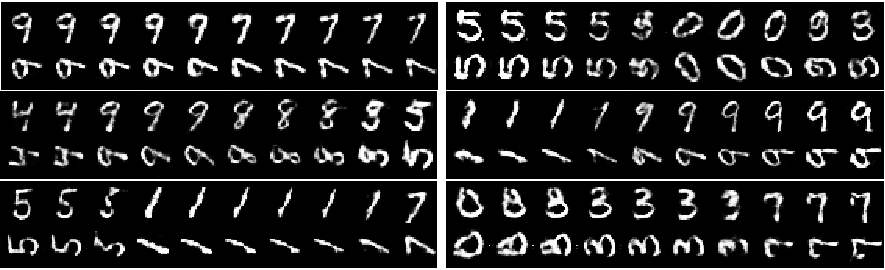
\includegraphics[trim=0.0in 0.0in 0.0in 0in, width=1.0\textwidth]{result_mnist_rotation.pdf}
\caption{Generation of digit and 90-degree rotated digit images. We visualized the CoGAN results by rendering pairs of images, using the vectors that corresponded to paths connecting two pints in the input noise space. For each of the sub-figures, the top row was from $\text{GAN}_1$ and the bottom row was from $\text{GAN}_2$. Each of the top and bottom pairs was rendered using the same input noise vector. We observed that CoGAN learned to synthesized corresponding digits with different rotation angles.}
\label{fig::result_mnist_rotation}
\end{figure}

\subsection{Weight Sharing}\label{subsec::sharing}

We analyzed the effect of weight sharing in the CoGAN framework. We conducted an experiment where we varied the numbers of weight-sharing layers in the generative and discriminative models to create different CoGAN architectures and trained them with the same hyperparameters. Due to lack of proper validation methods, we did a grid search on the training iteration and reported the best performance achieved by each network configuration for both Task $\mathbb{A}$ and $\mathbb{B}$\footnote{We noted that the performances were not sensitive to the number of training iterations.}. For each network architecture, we run 5 trails with different random network initialization weights. We then rendered 10000 pairs of images for each learned network. A pair of images consisted of an image in the first domain (generated by $\text{GAN}_1$) and an image in the second domain (generated by $\text{GAN}_2$), which were rendered using the same $\mathbf{z}$. 

For quantifying the performance of each weight-sharing scheme, we transformed the images generated by $\text{GAN}_1$ to the second domain by using the same method employed for generating the training images in the second domain. We then compared the transformed images with the images generated by $\text{GAN}_2$. The performance was measured by the average of the ratios of agreed pixels between the transformed image and the corresponding image in the other domain. Specifically, we rounded the transformed digit image to a binary image and we also rounded the rendered image in the second domain to a binary image. We then compared the pixel agreement ratio---the number of corresponding pixels that have the same value in the two images divided by the total image size. The performance of a trail was given by the pixel agreement ratio of the 10000 pairs of images. The performance of a network configuration was given by the average pixel agreement ratio over the 5 trails. We reported the performance results for Task $\mathbb{A}$ in Table~\ref{tbl::weight_sharing_analysis_A} and the performance results for Task $\mathbb{B}$ in Table~\ref{tbl::weight_sharing_analysis_B}.

From the tables, we observed that the pair image generation performance was positively correlated with the number of weight-sharing layers in the generative models. With more shared layers in the generative models, the rendered pairs of images were resembling more to true pairs drawn from the joint distribution. We noted that the pair image generation performance was uncorrelated to the number of weight-sharing layers in the discriminative models. However, we still preferred applying discriminator weight sharing because this reduces the total number of parameters. 

\begin{table}[thb!]
\centering
{
\caption{The table shows the performance of pair generation of digits and corresponding edge images (Task $\mathbb{A}$) with different CoGAN weight-sharing configurations. The results were the average pixel agreement ratios over 10000 images over 5 trials.}
\label{tbl::weight_sharing_analysis_A} 
\begin{tabular}{lc|cccc}
\hline
\multicolumn{2}{c|}{\multirow{2}{*}{Avg. pixel agreement ratio}} & \multicolumn{4}{c}{Weight-sharing layers in the generative models}\\
\multicolumn{2}{c|}{}   & 5 & 5,4 & 5,4,3 & 5,4,3,2\\
\hline
Weight-sharing &       & 0.894 $\pm$ 0.020	& 0.937 $\pm$ 0.004 &	0.943 $\pm$ 0.003 &	0.951 $\pm$ 0.004 \\
layers in the  & 4     & 0.904 $\pm$	0.018 & 0.939 $\pm$ 0.002 &	0.943 $\pm$ 0.005 &	0.950 $\pm$ 0.003 \\
discriminative & 4,3   & 0.888 $\pm$	0.036 & 0.934 $\pm$ 0.005 &	0.946 $\pm$ 0.003 &	0.941 $\pm$ 0.024 \\
models         & 4,3,2 & 0.903 $\pm$ 0.009 &	0.925 $\pm$ 0.021 &	0.944 $\pm$ 0.006 &	0.952 $\pm$ 0.002 \\
\hline
\end{tabular}}
\end{table}

\begin{table}[thb!]
\centering
{
\caption{The table shows the performance of pair generation of digits and corresponding negative images (Task $\mathbb{B}$) with different CoGAN weight-sharing configurations. The results were the average pixel agreement ratios over 10000 images over 5 trials.}
\label{tbl::weight_sharing_analysis_B} 
\begin{tabular}{lc|cccc}
\hline
\multicolumn{2}{c|}{\multirow{2}{*}{Avg. pixel agreement ratio}} & \multicolumn{4}{c}{Weight-sharing layers in the generative models}\\
\multicolumn{2}{c|}{}   & 5 & 5,4 & 5,4,3 & 5,4,3,2\\
\hline
Weight-sharing &       & 0.932 $\pm$ 0.011 & 0.946 $\pm$ 0.013 &	0.970 $\pm$ 0.002 &	0.979 $\pm$ 0.001 \\
layers in the  & 4     & 0.906 $\pm$ 0.066 & 0.953 $\pm$ 0.008 &	0.970 $\pm$ 0.003 &	0.978 $\pm$ 0.001 \\
discriminative & 4,3   & 0.908 $\pm$ 0.028 & 0.944 $\pm$ 0.012 &	0.965 $\pm$ 0.009 &	0.976 $\pm$ 0.001 \\
models         & 4,3,2 & 0.917 $\pm$ 0.022 & 0.934 $\pm$ 0.011 &	0.955 $\pm$ 0.010 & 0.969 $\pm$ 0.008 \\
\hline
\end{tabular}}
\end{table}

% \clearpage

\subsection{Comparison with the Conditional Generative Adversarial Nets}\label{subsec::cgan}



\begin{table}[thb!]
\small
\centering
{
\caption{Network architecture of the conditional GAN}
\label{tbl::cgan}
\begin{tabular}{|c|c|c|}
\hline\rule{0pt}{2ex}    
Layer &  Generative models \\
\hline 
input &  $\mathbf{z}$ and conditional variable $c\in\{0,1\}$ \\
1 &  FCONV-(N1024,K4x4,S1), BN, PReLU \\
2 &  FCONV-(N512,K3x3,S2), BN, PReLU \\
3 &  FCONV-(N256,K3x3,S2), BN, PReLU \\
4 &  FCONV-(N128,K3x3,S2), BN, PReLU \\
5 &  FCONV-(N1,K6x6,S1), Sigmoid \\
\hline
\hline\rule{0pt}{2ex} 
Layer &  Discriminative models \\
\hline\rule{0pt}{2ex} 
1 & CONV-(N20,K5x5,S1), POOL-(MAX,2) \\
2 & CONV-(N50,K5x5,S1), POOL-(MAX,2) \\
3 & FC-(N500), PReLU \\
4 & FC-(N3), Softmax \\
\hline
\end{tabular}}
\end{table}

\begin{table}[thb!]
\centering
{ 
\caption{Performance Comparison. For each task, we reported the average pixel agreement ratio scores and standard deviations over 5 trails, each trained with a different random initialization of the network connection weights.}
\label{tbl::cgan_perf}
\begin{tabular}{|c|c|c|}
\hline
Experiment & Task $\mathbb{A}$: Digit and Edge Images & Task $\mathbb{B}$: Digit and Negative Images \\
\hline
Conditional GAN & 0.909 $\pm$ 0.003 & 0.778 $\pm$ 0.021\\
CoGAN & {\bf 0.952} $\pm$ 0.002 & {\bf 0.967} $\pm$ 0.008\\
\hline
\end{tabular}}
\end{table}

\begin{figure}[thb!]
\centering
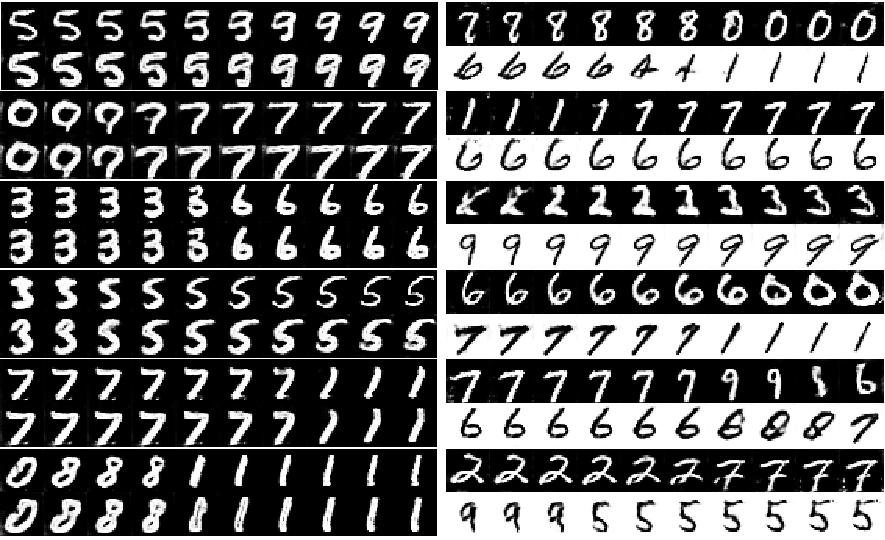
\includegraphics[trim=0.0in 0.0in 0.0in 0in, width=1.0\textwidth]{result_mnist_cgan.pdf}
\caption{Digit Generation with {\bf Conditional} Generative Adversarial Nets. Left:  generation of digit and corresponding edge images. Right: generation of digit and corresponding negative images. We visualized the conditional GAN results by rendering pairs of images, using the vectors that corresponded to paths connecting two pints in the input space. For each of the sub-figures, the top row was from the conditional GAN with the conditional variable set to 0, and the bottom row was from the conditional GAN with the conditional variable set to 1. That is each of the top and bottom pairs was rendered using the same input vector except for the conditional variable value. The conditional variable value was used to control the domain of the output images. From the figure, we observed that, although the conditional GAN learned to generate realistic digit images, it failed to learn the correspondence in the two domains. For the edge task, the conditional GAN rendered images of the same digits with a similar font. The edge style was not well-captured. For the negative image generation task, the conditional GAN simply failed to capture any correspondence. The rendered digits with the same input vector but different conditional variable values were not related. 
% This showed that the conditional GAN is not suited for learning to render corresponding images in a unsupervised fashion. On the contrary, the proposed CoGAN framework can learn to generate pairs of corresponding images without pairs of corresponding images in the training dataset as shown in Figure~\ref{fig::result_mnist_edge_vis}.
}
\label{fig::result_mnist_cgan_vis}
\end{figure}

We compared the CoGAN framework with the conditional generative adversarial networks (GAN) framework for joint image distribution learning. We designed a conditional GAN where the generative and discriminative models were identical to those used in the CoGAN in the digit experiments. The only difference was that the conditional GAN took an additional binary variable as input, which controlled the domain of the output image. The binary variable acted as a switch. When the value of the binary variable was zero, it generated images resembling images in the first domain. Otherwise, it generated images resembling those in the second domain. The output layer of the discriminative model was a softmax layer with three neurons. If the first neuron was on, it meant the input to the discriminative model was a synthesized image from the generative model. If the second neuron was on, it meant the input was a real image from the first domain. If the third neuron was on, it meant the input was a real image from the second domain. The goal of the generative model was to render images resembling those from the first domain when the binary variable was zero and to render images resembling those from the second domain when the binary variable was one. The details of the conditional GAN network architecture is shown in Table~\ref{tbl::cgan}.

Similarly to CoGAN learning, no correspondence was given during the conditional GAN learning. We applied the conditional GAN to the two digit generation tasks and hoped to answer whether a conditional model can be used to render corresponding images in two different domains without pairs of corresponding images in the training set. We used the same training data and hyperparameters as those used in the CoGAN learning. We trained the CoGAN for 25000 iterations\footnote{
We note the generation performance of the conditional GAN did not change much after 5000 iterations.} and used the trained network to render 10000 pairs of images in the two domains. Specifically, each pair of images was rendered with the same $\mathbf{z}$ but with different conditional variable values. These images were used to compute the pair image generation performance of the conditional GAN measured by the average of the pixel agreement ratios. For each task, we trained the conditional GAN for 5 times, each with a different random initialization of the network weights. We reported the average scores and the standard deviations.

The performance results are reported in Table~\ref{tbl::cgan_perf}. It can be seen that the conditional GAN achieved 0.909 for Task $\mathbb{A}$ and 0.778 for Task $\mathbb{B}$, respectively. They were much lower than the scores of 0.952 and 0.967 achieved by the CoGAN. Figure~\ref{fig::result_mnist_cgan_vis} visualized the conditional GAN's pair generation results, which suggested that the conditional GAN had difficulties in learning to render corresponding images in two different domains without pairs of corresponding images in the training set. 
% We then conclude that the conditional model is unable to learn a joint distribution from samples drawn separately from the marginal distributions of the individual domains.




\clearpage